\hspace*{0.6cm}
Энэ хэсэгт холимог микрофронтенд архитектурын хэрэгжүүлэлтийг тайлбарласан. Вэб хөгжүүлэлт нь HTML, CSS, JavaScript ашигладаг үеэс хол зам туулсан тул шаардлагатай хэрэгсэл, нөөц, хамаарал, статик файлууд илүү их эрэлт хэрэгцээтэй болсон. Иймд хялбараар вэб хөгжүүлэх, байршуулахын тулд боловсруулсан шинэ хэрэгслүүд нь орчин үеийн вэб хэрэглээний программ бүрийн чухал хэсэг бөгөөд энэ судалгааны ажилд тусгагдсан шийдлүүд юм.


\section{Туршилтын загварын бүтэц}
\label{sec:prototype}
Туршилтын загвар нь Оюутны жагсаалт микрофронтенд болон Сэдвийн сан микрофронтендээс бүрдэнэ. Микрофронтенд бүрийг Үндсэн аппликейшн рүү ачаалдаг. Зураг \ref{fig:prototype-structure}-т туршилтын загварын бүтцийг харуулав. Туршилтын загварыг боловсруулахын тулд хийгдсэн алхмуудыг төслийн бүтэц, Webpack тохиргоо, техникийн орчин хүртэл дэлгэрэнгүй тайлбарласан.
\begin{figure}[H]
	\centering
	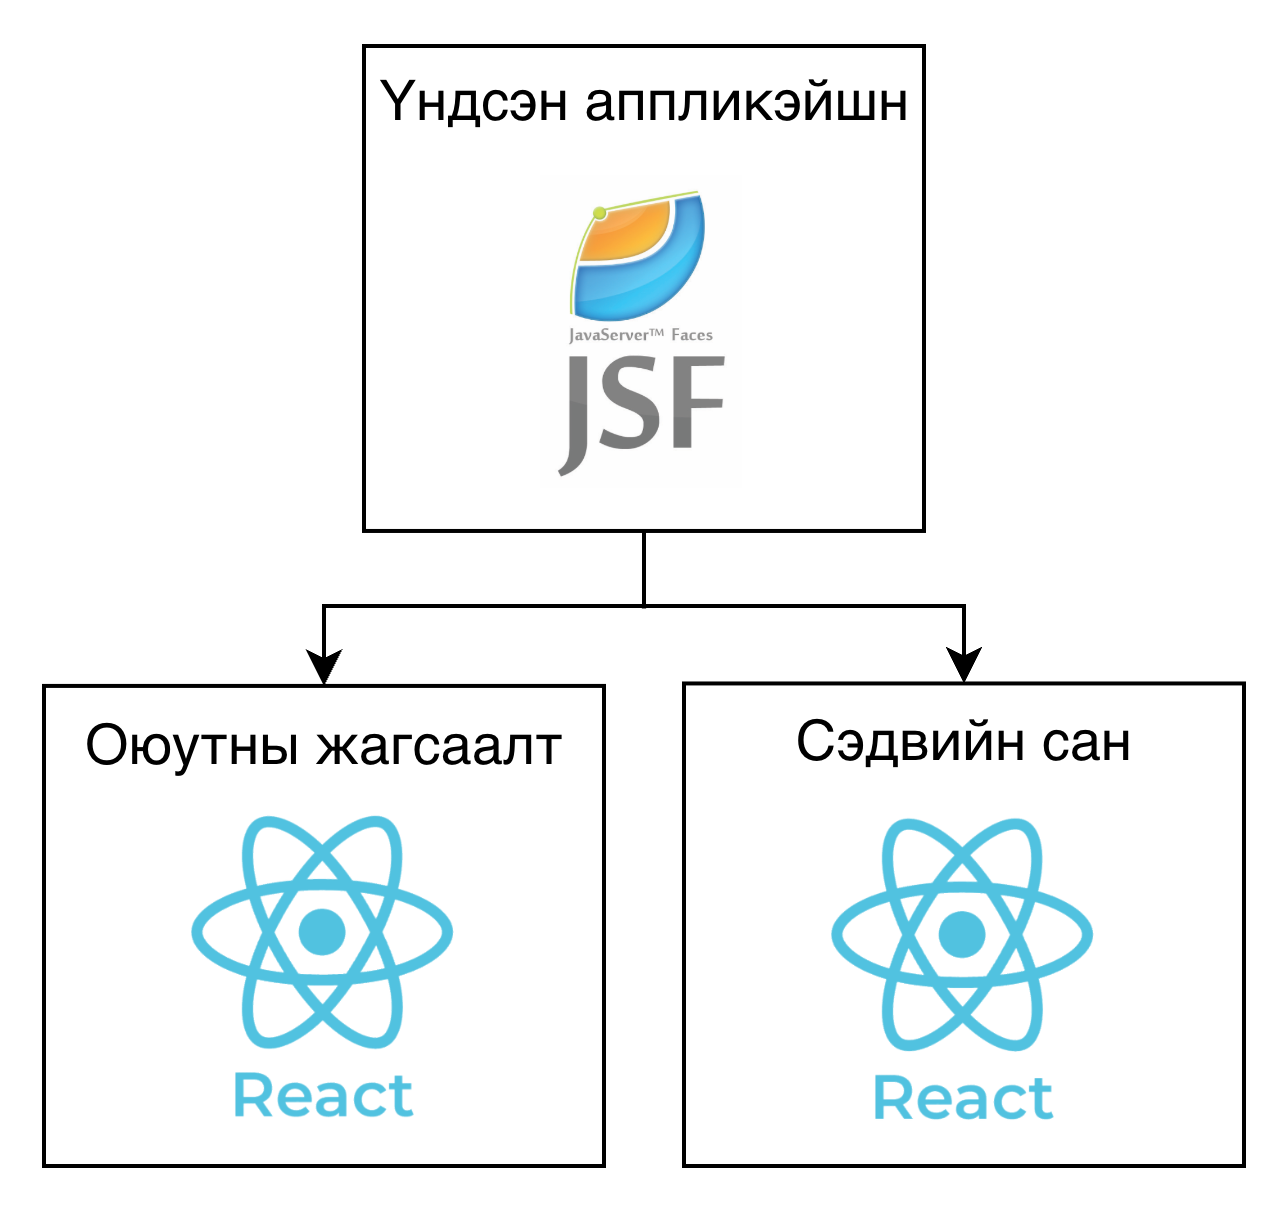
\includegraphics[width=9cm]{images/prototype-structure.png}
	\caption{Туршилтын загварын бүтэц}
	\label{fig:prototype-structure}
\end{figure}
Туршилтын загварын бүтэц нь Үндсэн хэрэглээний программ, Микрофронтенд модулиуд гэсэн үндсэн бүрэлдэхүүн хэсгүүдээс бүрдэнэ. Үндсэн хэрэглээний программ нь дотроо React хэрэглээний программуудыг ачааллах зориулалттай хоосон DOM элементүүдийг бэлтгэж өгнө. Туршилтын загварыг хөгжүүлэхэд ашигласан технологиудын хувилбарыг Хүснэгт \ref{tab:tech-env}-д харуулав.
\begin{table}[H]
\centering
\caption{Туршилтын загварын техникийн орчин}
\label{tab:tech-env}
\renewcommand{\arraystretch}{1}
\begin{tabular}{lccc}
\toprule
\textbf{Технологи} & \textbf{Үндсэн хэрэглээний программ} & \textbf{Модуль 1} & \textbf{Модуль 2} \\ 
\midrule
Node.js & - & 18.18.0 & 18.18.0 \\ 
Webpack & - & 5.81.0 & 5.81.0 \\ 
JSF & 2.3 & - & - \\ 
React & - & 18.2.0 & 18.2.0 \\ 
\bottomrule
\end{tabular}
\end{table}
% \section{JavaServer Faces}

% JavaServer Faces (JSF) нь Java EE стандартын нэг хэсэг бөгөөд вэб хэрэглээний программын хэрэглэгчийн интерфэйсийг бүрэлдэхүүн хэсэгт суурилан хөгжүүлэх боломжийг олгодог серверийн талын фреймворк юм. Хөтөч дээр ажилладаг орчин үеийн SPA архитектураас ялгаатай нь JSF нь серверийн талд хөрвүүлэлт хийх үндсэн зарчимтай ажилладаг. JSF-ийн гол онцлогуудыг доорх гурван хэсэгт хуваан авч үзэж болно.

% \subsection{Серверийн талын хөрвүүлэлт ба Facelets}
% \hspace*{0.6cm}Хэрэглэгчээс хөтчөөр дамжуулан хүсэлт (HTTP Request) илгээх үед JSF нь тухайн хуудасны \texttt{Facelets} (\texttt{.xhtml}) загварын хуудсыг сервер дээр уншиж боловсруулдаг. Түүн доторх JSF-ийн тусгай тагуудыг (жишээлбэл \texttt{<h:inputText>}, \texttt{<h:dataTable>}) стандарт HTML, CSS болон шаардлагатай JavaScript код руу хөрвүүлэн угсардаг. Үүний дараа бүрэн боловсруулагдсан, эцсийн цэвэр HTML баримтыг хөтөч рүү буцаадаг (HTTP Response). Иймд хөтөч нь зөвхөн бэлэн болсон HTML-ийг зурж харуулах үүрэг хүлээх бөгөөд хуудасны үндсэн төлөв сервер дээр хадгалагддаг.

% \subsection{Төлөвийн удирдлага ба Managed Beans}
% \hspace*{0.6cm}JSF-ийн бас нэгэн гол онцлог нь UI элементүүд болон серверийн талын Java объектуудын (Managed Beans буюу Backing Beans) хооронд өгөгдлийн хоёр чиглэлт холбоос үүсгэдэг явдал юм. Хэрэглэгчийн оруулсан өгөгдөл эсвэл товч дарах үйлдэл нь шууд серверийн талд байгаа Java функцүүдтэй холбогдон ажжилладаг. Үүний тулд JSF нь тухайн хуудасны төлөвийг тусгай Component Tree бүтцээр санах ойд эсвэл хөтчийн нуугдмал талбарт хадгалж, дараагийн хүсэлт ирэх үед бүтцийг өмнөх байдалд нь сэргээж ажилладаг.

% \subsection{Хүсэлт боловсруулах амьдралын мөчлөг}
% \hspace*{0.6cm}Хэрэглэгчийн хийсэн үйлдэл бүрийг JSF нь маш нарийн тодорхойлогдсон 6 үе шаттай мөчлөгөөр боловсруулдаг. Үүнд:
% \begin{itemize}
%     \item Хүсэлт хүлээн авч, хуудасны Component бүтцийг сэргээх.
%     \item Хэрэглэгчийн оруулсан утгуудыг хуудасны элементүүдэд олгох.
%     \item Өгөгдлийн үнэн зөв байдал ба баталгаажуулалт хийх.
%     \item Батлагдсан өгөгдлөөр серверийн объектын утгыг шинэчлэх.
%     \item Хэрэглэгчийн үйлдлийг буюу үндсэн Java логикийг ажиллуулах.
%     \item Эцсийн HTML баримтыг үүсгэж хөтөч рүү илгээх.
% \end{itemize}

% Дээр дурдсанчлан JSF нь аюулгүй байдал өндөртэй, сервер талд өгөгдлөө найдвартай удирддаг давуу талтай хэдий ч, UI хэсгийг динамикаар хурдан өөрчлөх эсвэл орчин үеийн баялаг интерактив үйлдэл нэмэх үед хуудсыг байнга дахин ачаалах шаардлага гарах зэрэг хязгаарлалттай тулгардаг. Тиймээс энэхүү төслийн архитектурт JSF-ийн бат бөх суурь болох өгөгдлийн хамгаалалт, чиглүүлэлтийг хэвээр үлдээж, хэрэглэгчийн өндөр интерактив үйлдэл шаардсан хэсгүүдэд микрофронтендийг хөтөч дээр скрипт (\texttt{<script>}) байдлаар нэгтгэн суулгах архитектурын шийдлийг сонгосон болно.

% \section{Webpack тохиргоо ба Интеграци}

% Орчин үеийн JavaScript фреймворкууд нь хөгжүүлэлтийн орчноо Webpack хэрэгсэлд суурилан бүрдүүлдэг бөгөөд төслийн скриптүүдийг \texttt{package.json} файлд тохируулдаг. Зураг \ref{fig:package-update}-д үзүүлснээр \texttt{"start"} болон \texttt{"build"} скриптүүдийн тусламжтайгаар микрофронтенд модулиудыг хөгжүүлэлтийн орчинд бие даан ажиллуулах боломжтойг харуулав. Энэхүү туршилтын загварт React модулиудыг JSF-тэй нэгтгэхдээ Webpack Module Federation (WMF) бус, харин хөтчөөс \texttt{<script>} таг ашиглан динамикаар ачааллах (Script Injection) аргыг сонгон хэрэгжүүлсэн. 

% Уг шийдлийн хүрээнд JSF хостын \texttt{.xhtml} хуудас хөтчид бүрэн ачаалагдсаны дараа Webpack-аар багцлагдсан \texttt{main.js} файлыг дуудан, \texttt{\#microfrontend-root} DOM элемент дотор React хэрэглээний программыг дүрслэх (render) зарчмаар ажиллана. Энэ нь \ref{sec:integration-types} хэсэгт дурдсан ажиллах үеийн (run-time) интеграцийн зарчимд бүрэн нийцэж байгаа юм. React модуль тус бүр бие даан багцлагддаг тул JSF хост хэрэглээний программынн кодод өөрчлөлт оруулахгүйгээр тусад нь байршуулах (deploy) боломжтой бөгөөд энэ нь системийн сул хамааралтай (loose coupling) байдлыг хангаж байна.

% Микрофронтенд архитектурт түгээмэл ашиглагддаг WMF аргачлалаас татгалзаж, Script Injection аргыг сонгосон нь техникийн болон архитектурын хувьд дараах үндэслэлтэй. WMF нь үндсэндээ хост болон дэд (remote) хэрэглээний программууд нь хоёулаа JavaScript технологид суурилсан орчинд хоорондоо холбогдон ажиллахад илүү зохицдог. Харин энэхүү системийн үндсэн хост нь серверийн талд HTML хуудсыг боловсруулдаг Java (JSF) технологи тул тэс өөр архитектуртай орчинд WMF-ийг нэвтрүүлэх нь системийн тохиргоог хүндрүүлж, зохиомжийн нийлмэл байдлыг (complexity) шаардлагагүйгээр нэмэгдүүлэх сул талтай.

% Үүний эсрэгээр Script Injection аргыг ашигласнаар JSF нь \texttt{.xhtml} хуудсаа серверээс боловсруулан гаргасны дараа хөтөч тухайн React-ийн багцлагдсан \texttt{main.js} файлыг бие даан уншиж, ажиллуулах боломж бүрдсэн. Энэхүү хандлага нь хост болон микрофронтенд хоорондын технологийн хамаарлыг (dependency) хамгийн бага түвшинд барих бөгөөд архитектурын хувьд илүү энгийн, найдвартай интеграцийн шийдэл болж чадсан болно.

% \begin{figure}[H]
% 	\centering
% 	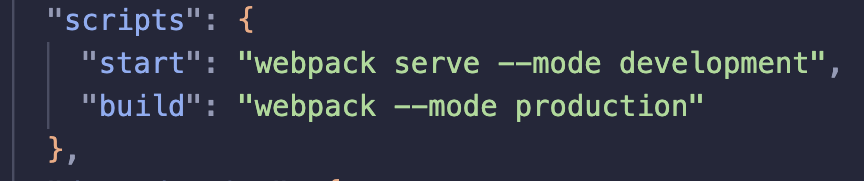
\includegraphics[width=12cm]{images/package-update.png}
% 	\caption{Package.json өөрчлөлт}
% 	\label{fig:package-update}
% \end{figure}

\section{Асинхрон скрипт ачаалалт}
Микрофронтендүүдийг ачааллах үед шаардлагатай хамаарал бүрэн татагдаж дуусаагүй байхад хэрэглээний программ уншигдаж эхэлбэл алдаа гарах эрсдэлтэй. Үүнээс сэргийлэхийн тулд асинхрон скрипт ачаалалтыг ашигласан. Хэрэглээний программыг эхлүүлэх логикийг \texttt{bootstrap.js} файл дотор бичиж, \texttt{index.js} нь зөвхөн \texttt{import('./bootstrap');} гэсэн динамик дуудлагыг агуулна. Webpack энэ динамик дуудлагыг хөрвүүлэх явцад кодыг хэд хэдэн chunk файл болгон хуваадаг: \texttt{main.js} нь оролтын файл бөгөөд \texttt{bootstrap.js}-г агуулсан chunk болон React vendor chunk-уудыг динамикаар дуудна. Иймд \texttt{webpack.config.js} файл дотор \texttt{output} \texttt{.publicPath}-ийг зөв тохируулах шаардлагатай бөгөөд энэ нь хөтчид chunk файлуудыг зөв замаас татах боломжийг олгоно.
\begin{figure}[H]
	\centering
	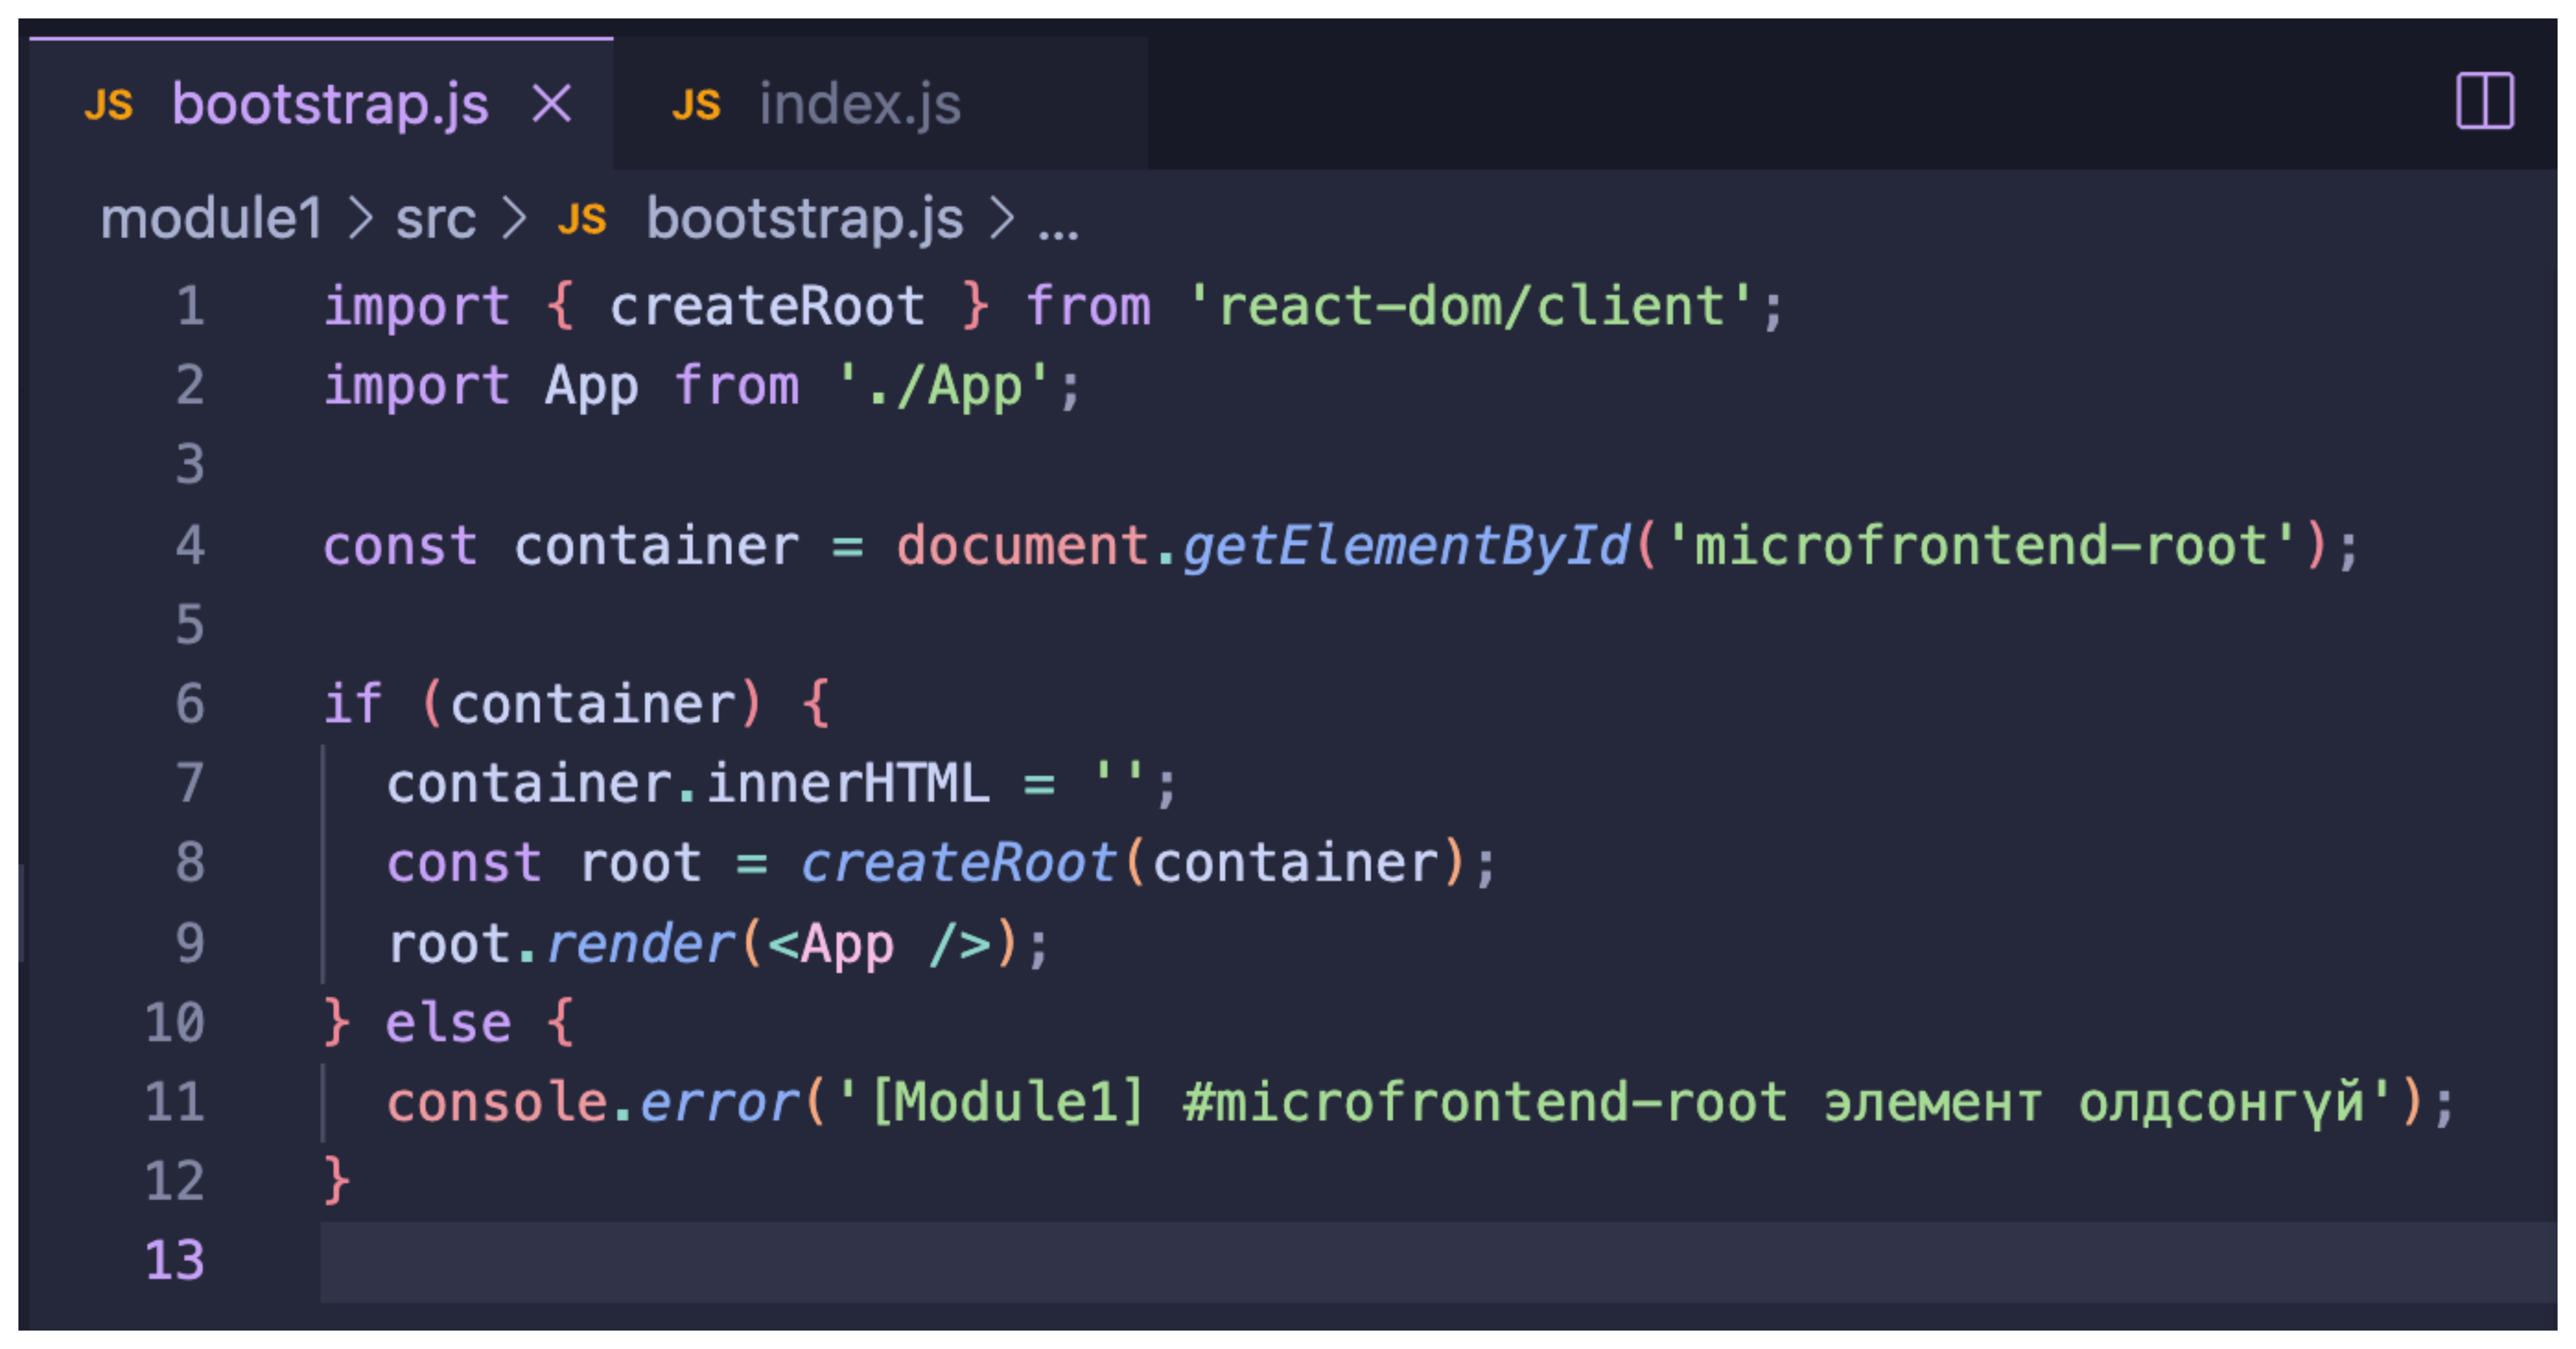
\includegraphics[width=14cm]{images/async-1.png}
	\caption{Асинхрон скрипт ачаалалтын эхлүүлэх логик}
	\label{fig:async-1}
\end{figure}
\begin{figure}[H]
	\centering
	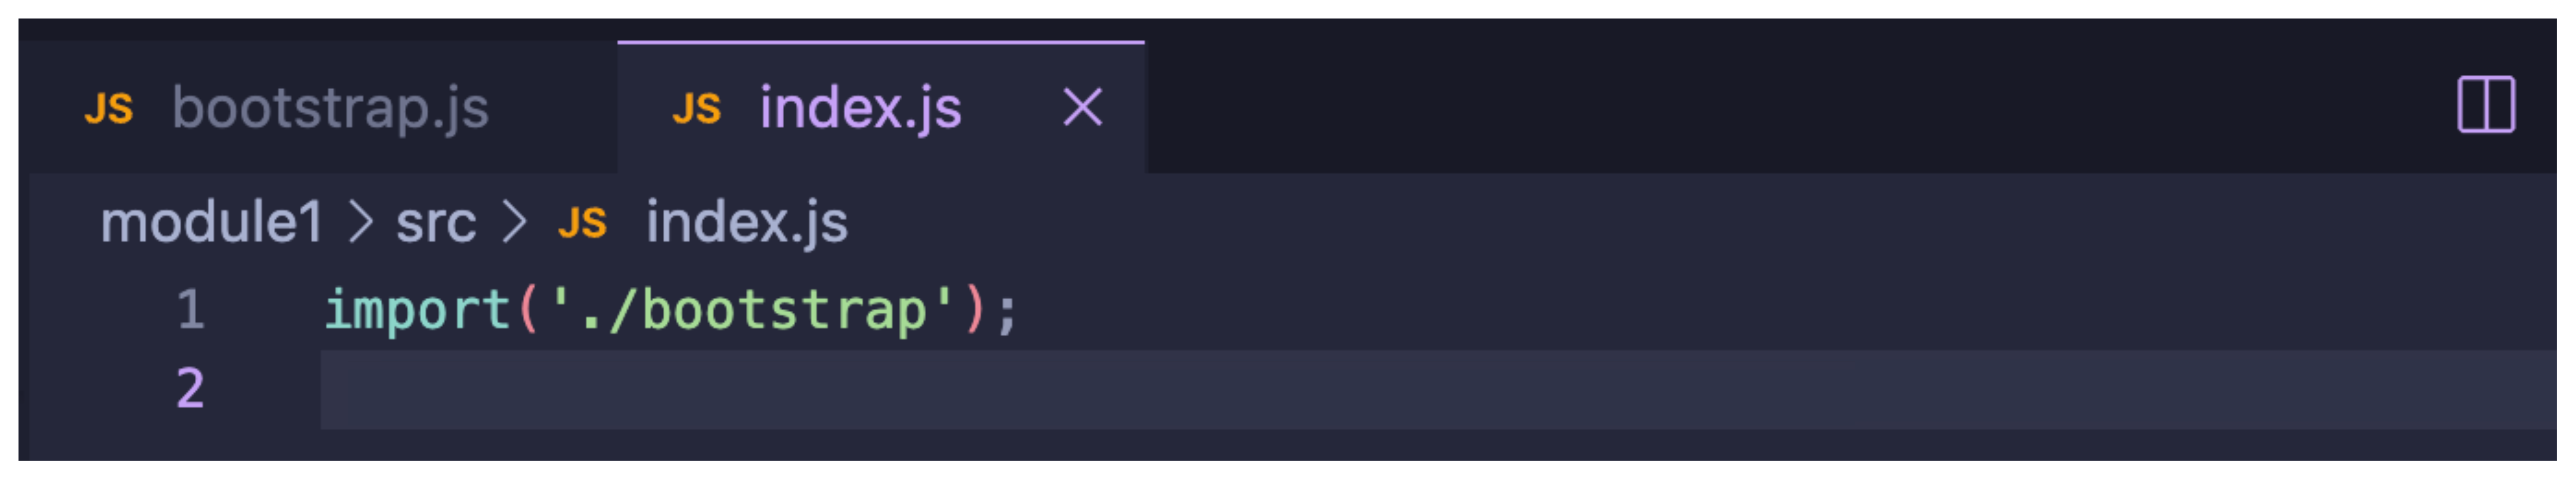
\includegraphics[width=14cm]{images/async-2.png}
	\caption{Асинхрон скрипт ачаалалтын динамик дуудлага}
	\label{fig:async-2}
\end{figure}

\section{CSS загварын давхцал}
Хэрэглэгч нэг микрофронтендийн хуудаснаас нөгөө рүү шилжих үед хөтөч нь тухайн модулиудын CSS загваруудыг DOM-ийн \texttt{<head>} хэсэгт нэмж ачаалдаг бөгөөд ижил нэртэй CSS классууд нэгнийгээ дарж бичин, UI-ийн хэв гажилт үүсгэдэг байна. Энэ асуудлаас сэргийлэхийн тулд туршилтын загварт CSS Modules аргачлалыг ашигласан. Модуль бүрийн загварын файлыг \texttt{.module.css} өргөтгөлтэйгээр үүсгэж, \texttt{webpack.config.js} дотор \texttt{css-loader}-ын \texttt{modules} тохиргоог идэвхжүүлсэн. Webpack хөрвүүлэлтийн явцад CSS класс бүрийн нэрэнд \texttt{[name]\_[local]\_[hash:6]} загварын дагуу давтагдахгүй хэш утга залгадаг тул JSF үндсэн хэрэглээний программ болон бусад React модулиудын загвартай мөргөлдөхөөс бүрэн хамгаалагддаг.

Хэдийгээр CSS Modules нь React компонентүүдийн класс нэрийг дахин давтагдашгүй болгож, тэднийг бусад модуль болон JSF хэсэгтэй мөргөлдөхөөс бүрэн хамгаалдаг боловч нэгэн техникийн хязгаарлалт байдгийг дурдах нь зүйтэй. JSF хост хэрэглээний программын талд тодорхойлогдсон глобал загварууд нь React компонентүүд рүү доошоо уламжлагдан орж ирж нөлөөлөх эрсдэл бий. Учир нь JSF болон React нь хөтөч дээр нэг л DOM модонд хамтдаа байрладаг. 

Энэ глобал нөлөөллөөс сэргийлж тусгаарлахын тулд Web Components стандартын нэг хэсэг болох \textit{Shadow DOM} ашиглах хувилбарыг онолын хувьд давхар судалсан. Гэвч Shadow DOM-ийг React-тэй хоршуулан ашиглах үед Webpack-ийн \texttt{style-loader}-ийн тохиргоог хэт хүндрүүлдэг төдийгүй, дэлгэцийн хүрээнээс гадуур дүрслэгддэг React Portals (жишээ нь Modal, Dialog, Tooltip) суурьтай 3-дагч UI компонентүүдийн загвар алдагдаж эвдрэх өндөр магадлалтай байдаг. Тиймээс хост болон микрофронтендийн кодыг нэг дор удирдан хөгжүүлж буй энэхүү туршилтын нөхцөлд CSS Modules аргачлал нь архитектурын хувьд хавьгүй оновчтой бөгөөд хөнгөн шийдэл болно гэж дүгнэн сонгосон болно.

\begin{figure}[H]
	\centering
	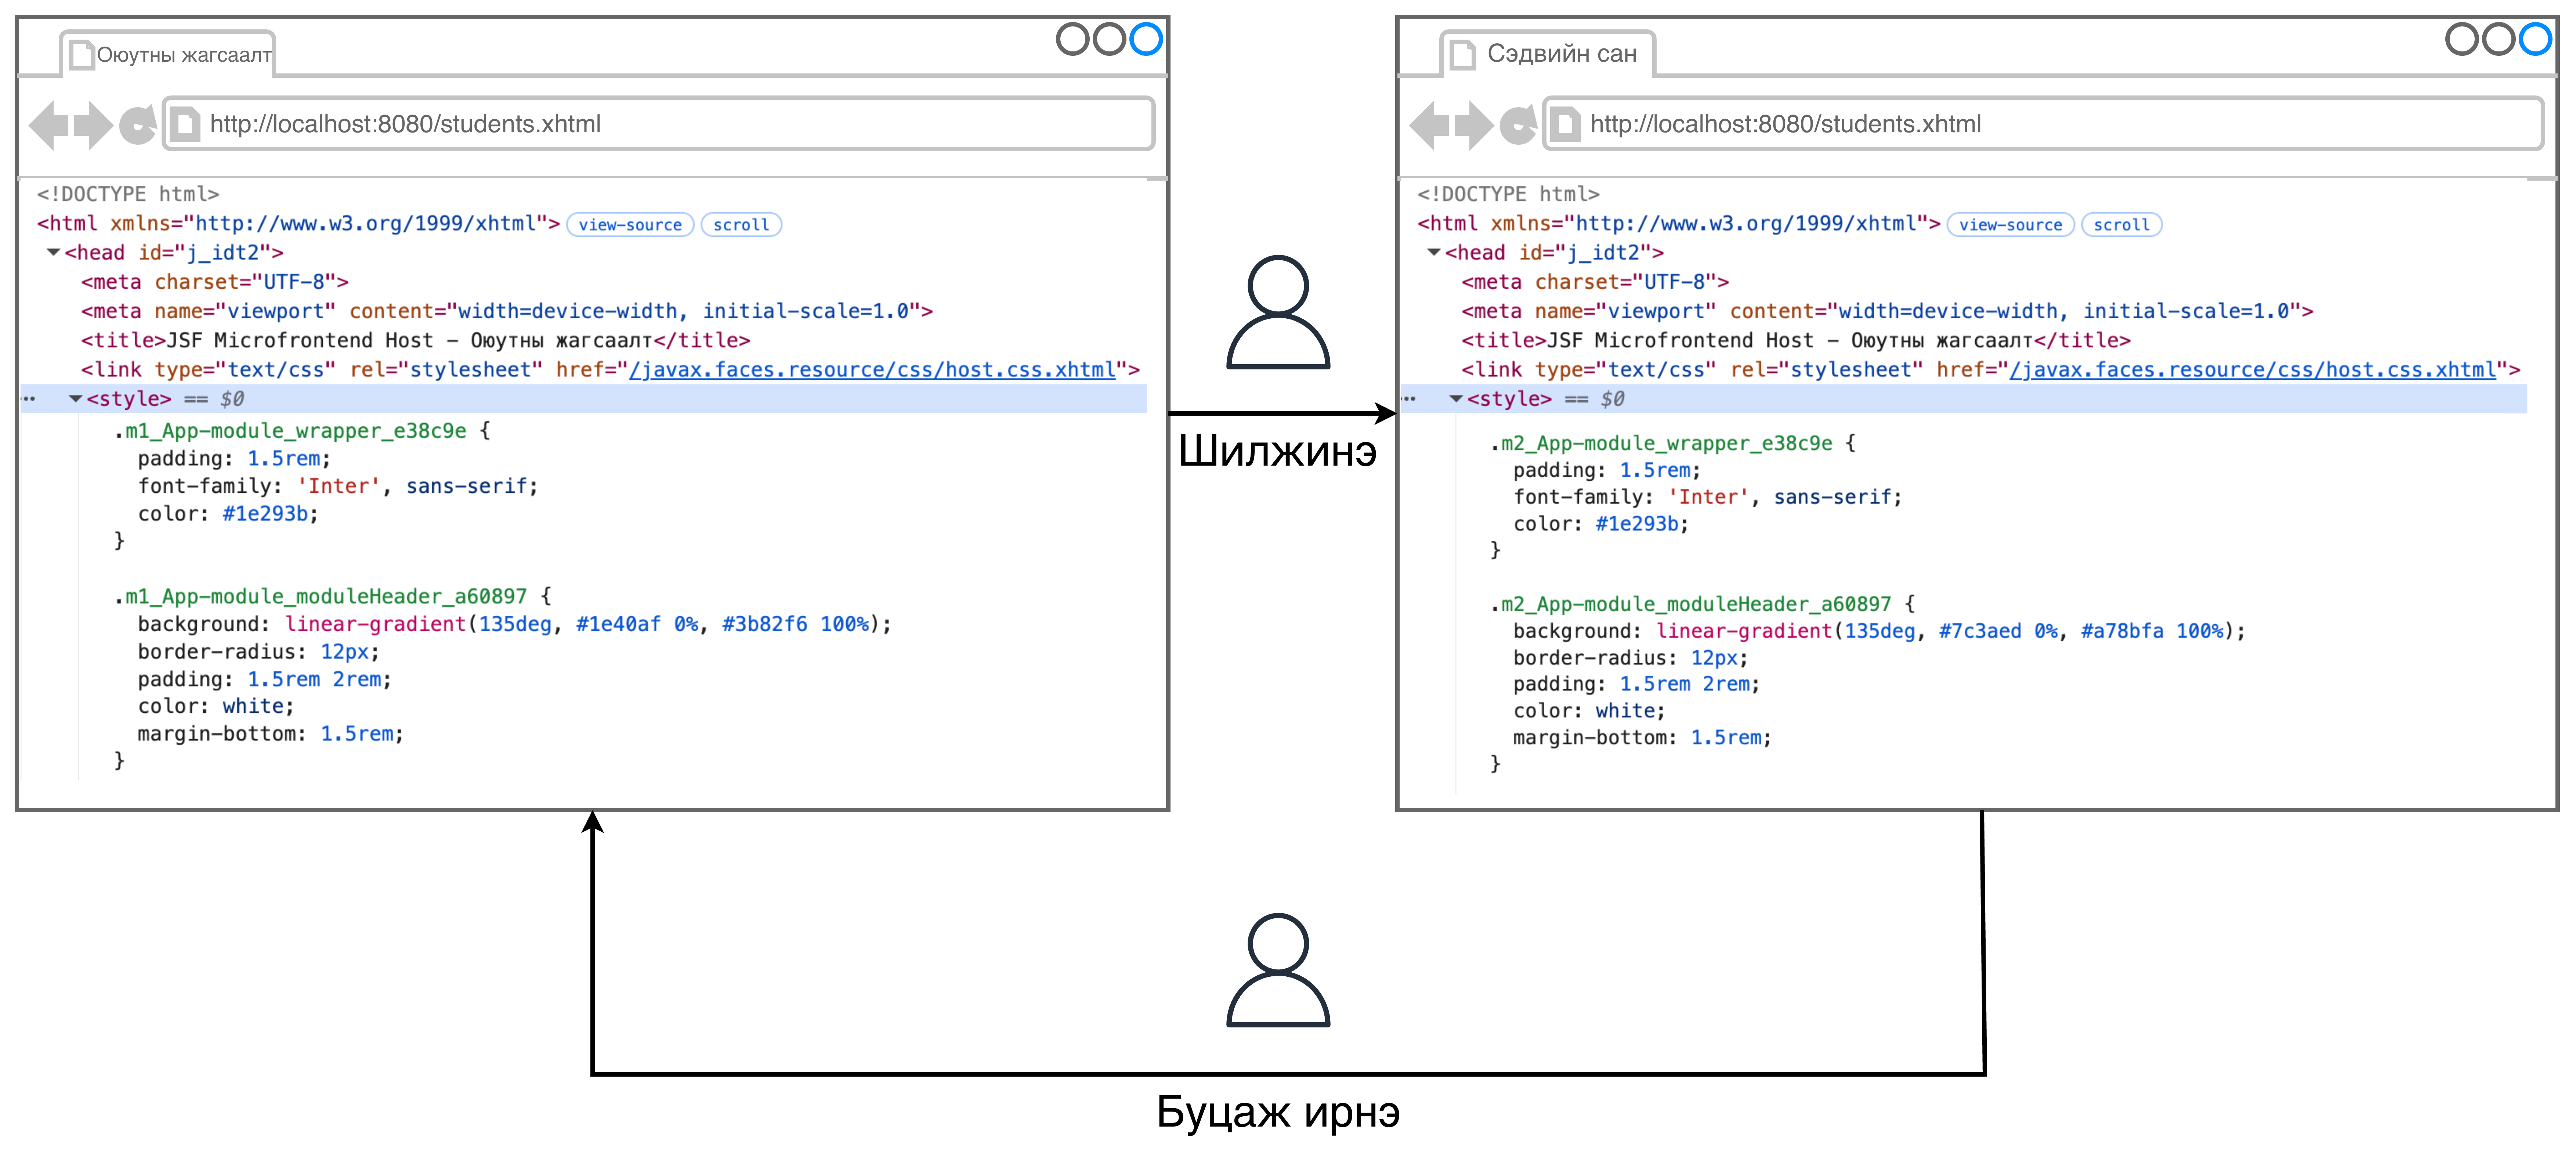
\includegraphics[width=15cm]{images/css-modules.png}
	\caption{CSS Modules-ийн хэш нэмэгдсэн класс нэрүүд (Browser DevTools)}
	\label{fig:css-modules}
\end{figure}

% \section{Туршилт}
% \label{sec:experiment}
% Энэхүү туршилтын зорилго нь уламжлалт JSF системд React микрофронтенд модулиудыг нэгтгэсэн холимог архитектурыг бодитоор хэрэгжүүлж, түүний техникийн боломж, үр ашгийг одоогийн цэвэр микрофронтенд архитектуртай харьцуулан судлахад оршино. Түүнчлэн бодит бизнес процесст тулгуурлан микрофронтенд модулиудын хил хязгаарыг зөв тодорхойлох нь туршилтын чухал хэсэг юм.

\subsection{Одоо байгаа шийдэл}
Орчин үеийн цэвэр микрофронтенд архитектурын нийтлэг шийдлийг Зураг \ref{fig:mfe}-т харуулав. Энэхүү бүтэц нь дан ганц React гэх мэт орчин үеийн фреймворк дээр суурилсан үндсэн хэрэглээний программ болон бие даасан микрофронтенд модулиудаас бүрддэг. Модуль тус бүр нь бэкенд дэх өөрийн харгалзах микросервисээр дамжуулан тусгаарлагдсан өгөгдлийн сантай харилцдаг. Энэ нь цоо шинээр хөгжүүлэгдэж буй системүүдэд маш тохиромжтой хэдий ч, олон жил ашиглагдсан, бизнесийн цогц логик бүхий JSF суурьтай цул системийг тэр чигт нь энэхүү архитектур руу шууд шилжүүлэхэд хөгжүүлэлтийн цаг хугацаа болон нөөцийн хувьд хэт өндөр зардалтай юм.

\begin{figure}[H]
  \centering
  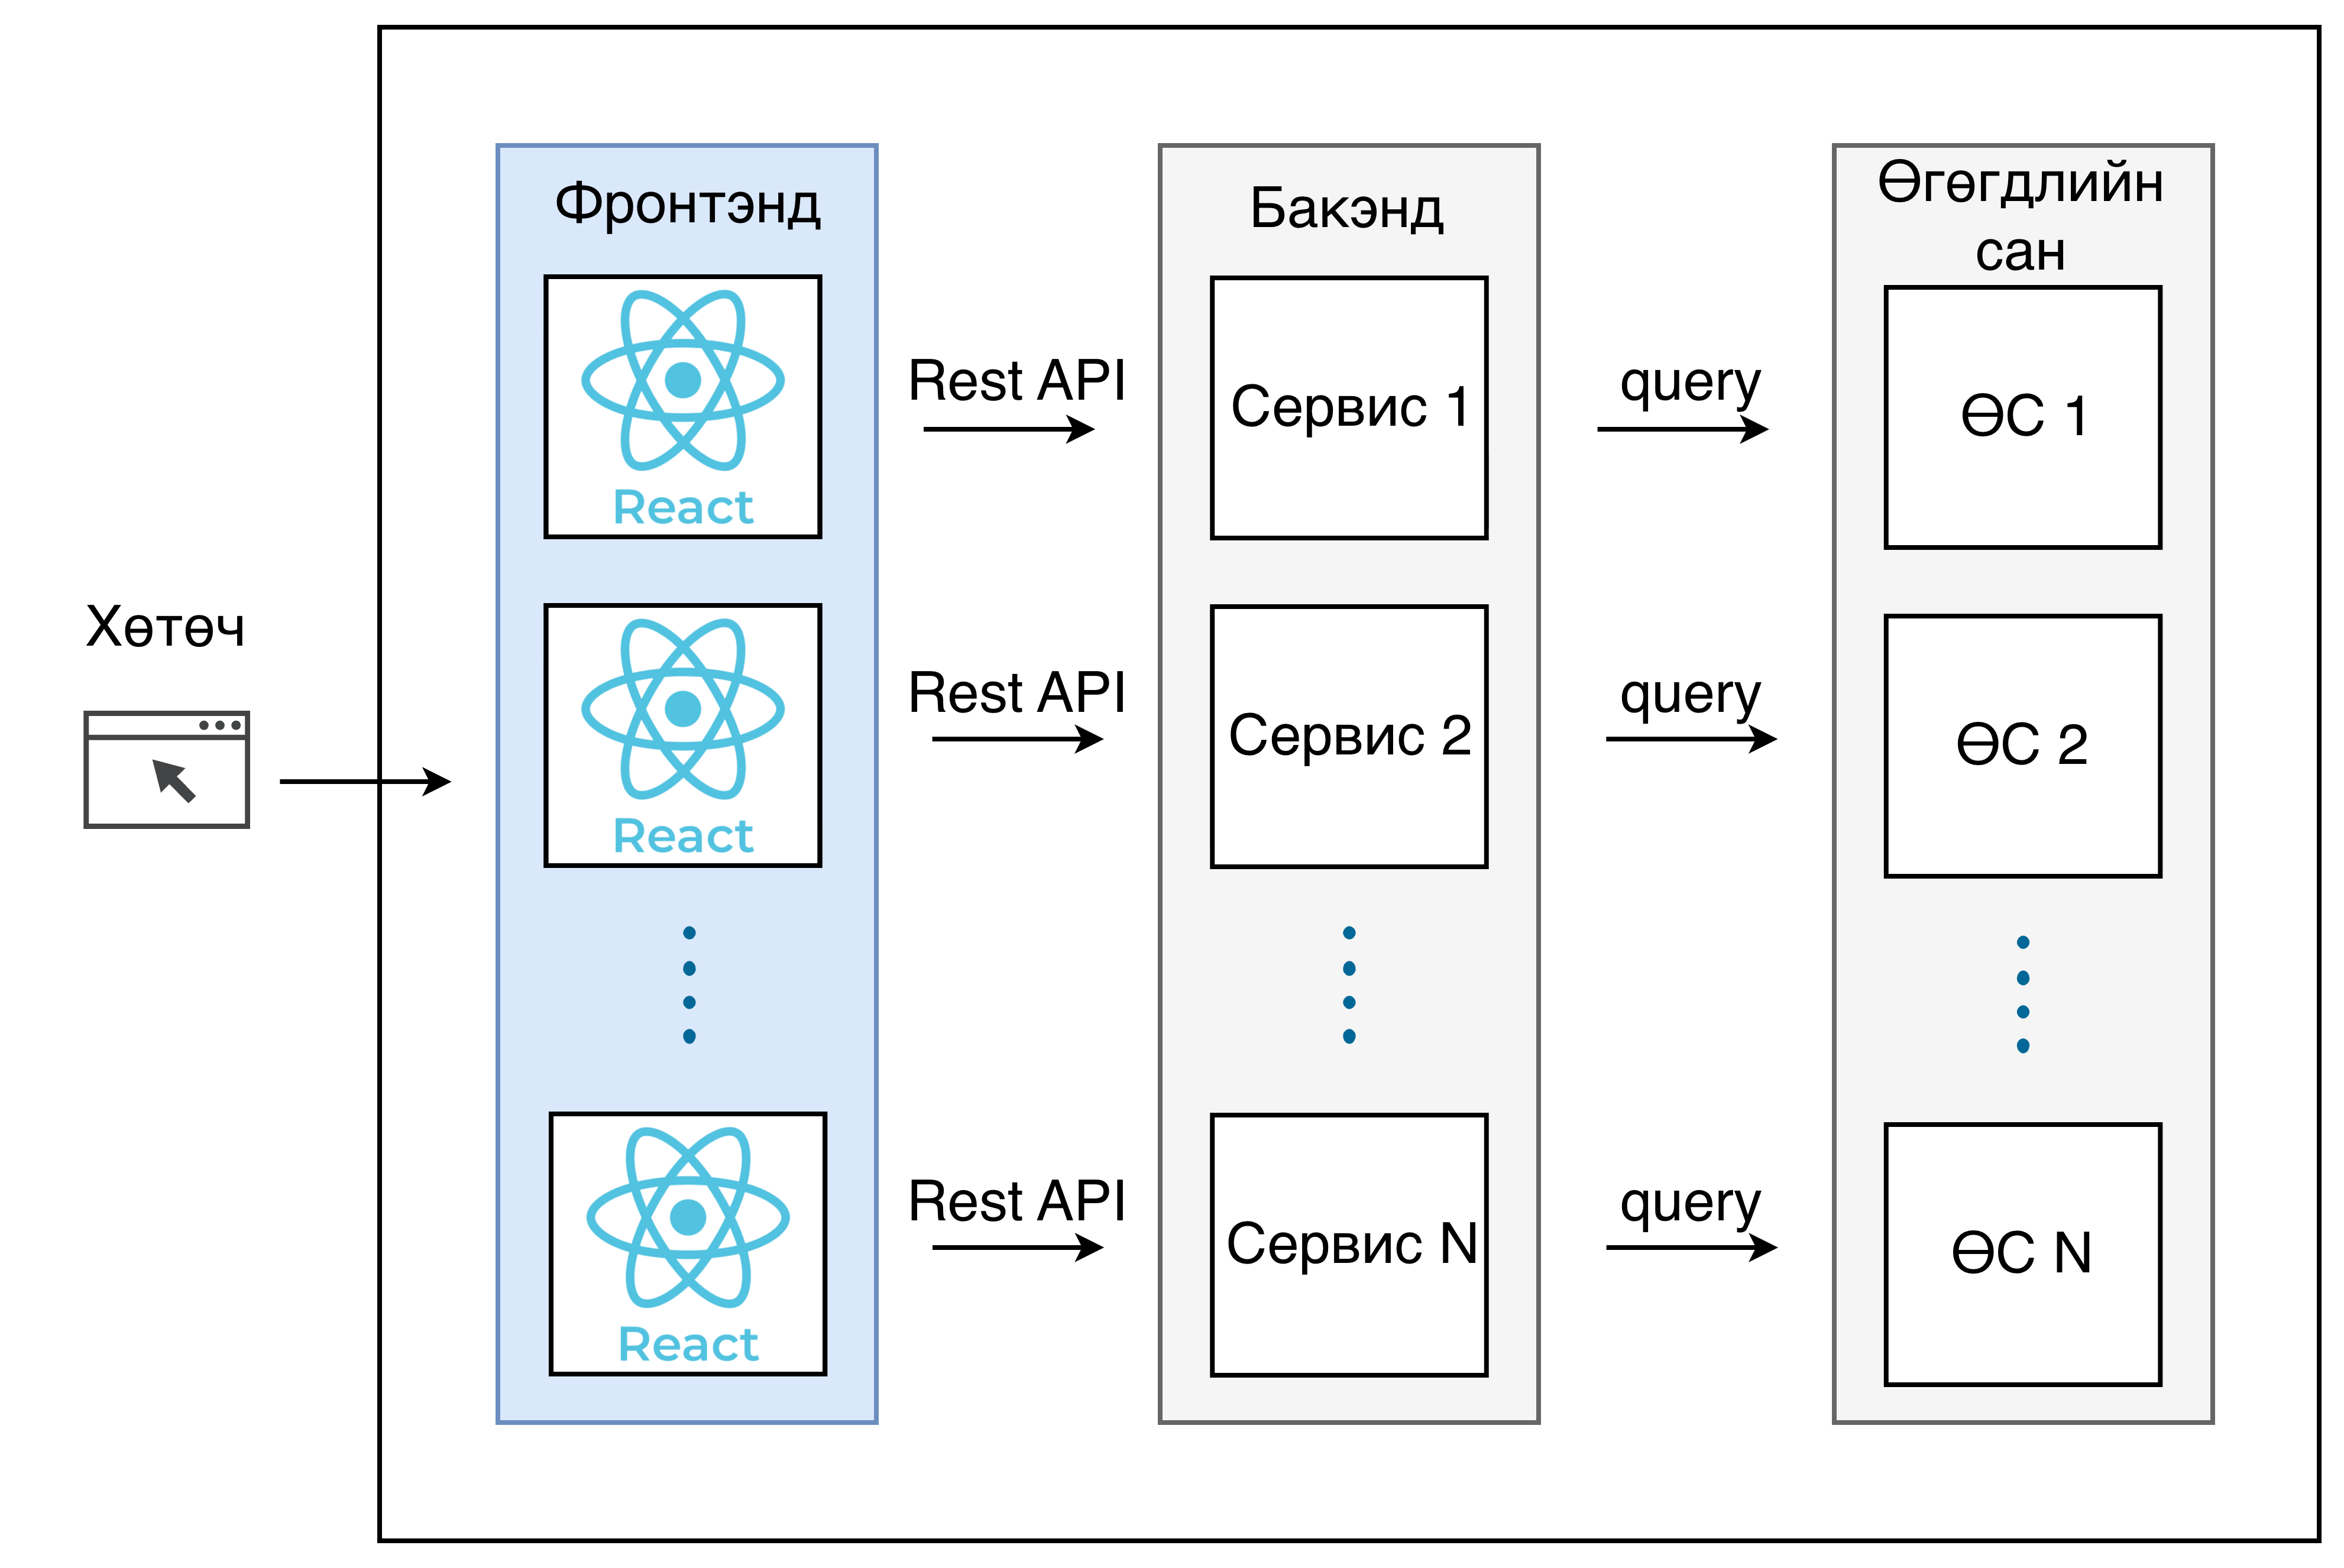
\includegraphics[width=10cm]{images/mfe.png}
  \caption{Одоо байгаа микрофронтенд архитектурын шийдэл}
  \label{fig:mfe}
\end{figure}

\subsection{Санал болгож буй шийдэл}
Уламжлалт системийг шинэчлэхэд үүсдэг дээрх хүндрэлийг шийдвэрлэхийн тулд Зураг \ref{fig:hybrid-mfe}-т үзүүлсэн холимог микрофронтенд архитектурыг энэхүү судалгаагаар санал болгож байна. Энэхүү шийдэл нь хуучин JSF хэрэглээний программыг бүрэн устгахын оронд, түүнийг хэрэглэгчийн интерфейсийн эх бие буюу хост болгон ашиглах зарчимд тулгуурлана. Шинээр хөгжүүлэх шаардлагатай модулиудыг React фреймворкоор бие даан хөгжүүлж, JSF-ийн хуудсанд \texttt{<script>} тагаар динамикаар нэгтгэнэ. Ингэснээр хуучин системийн тогтвортой ажиллагааг хадгалахын зэрэгцээ, орчин үеийн технологийн давуу талыг ашиглан системийг үе шаттайгаар, эрсдэл багатайгаар шинэчлэх боломж бүрдэх юм.

\begin{figure}[H]
  \centering
  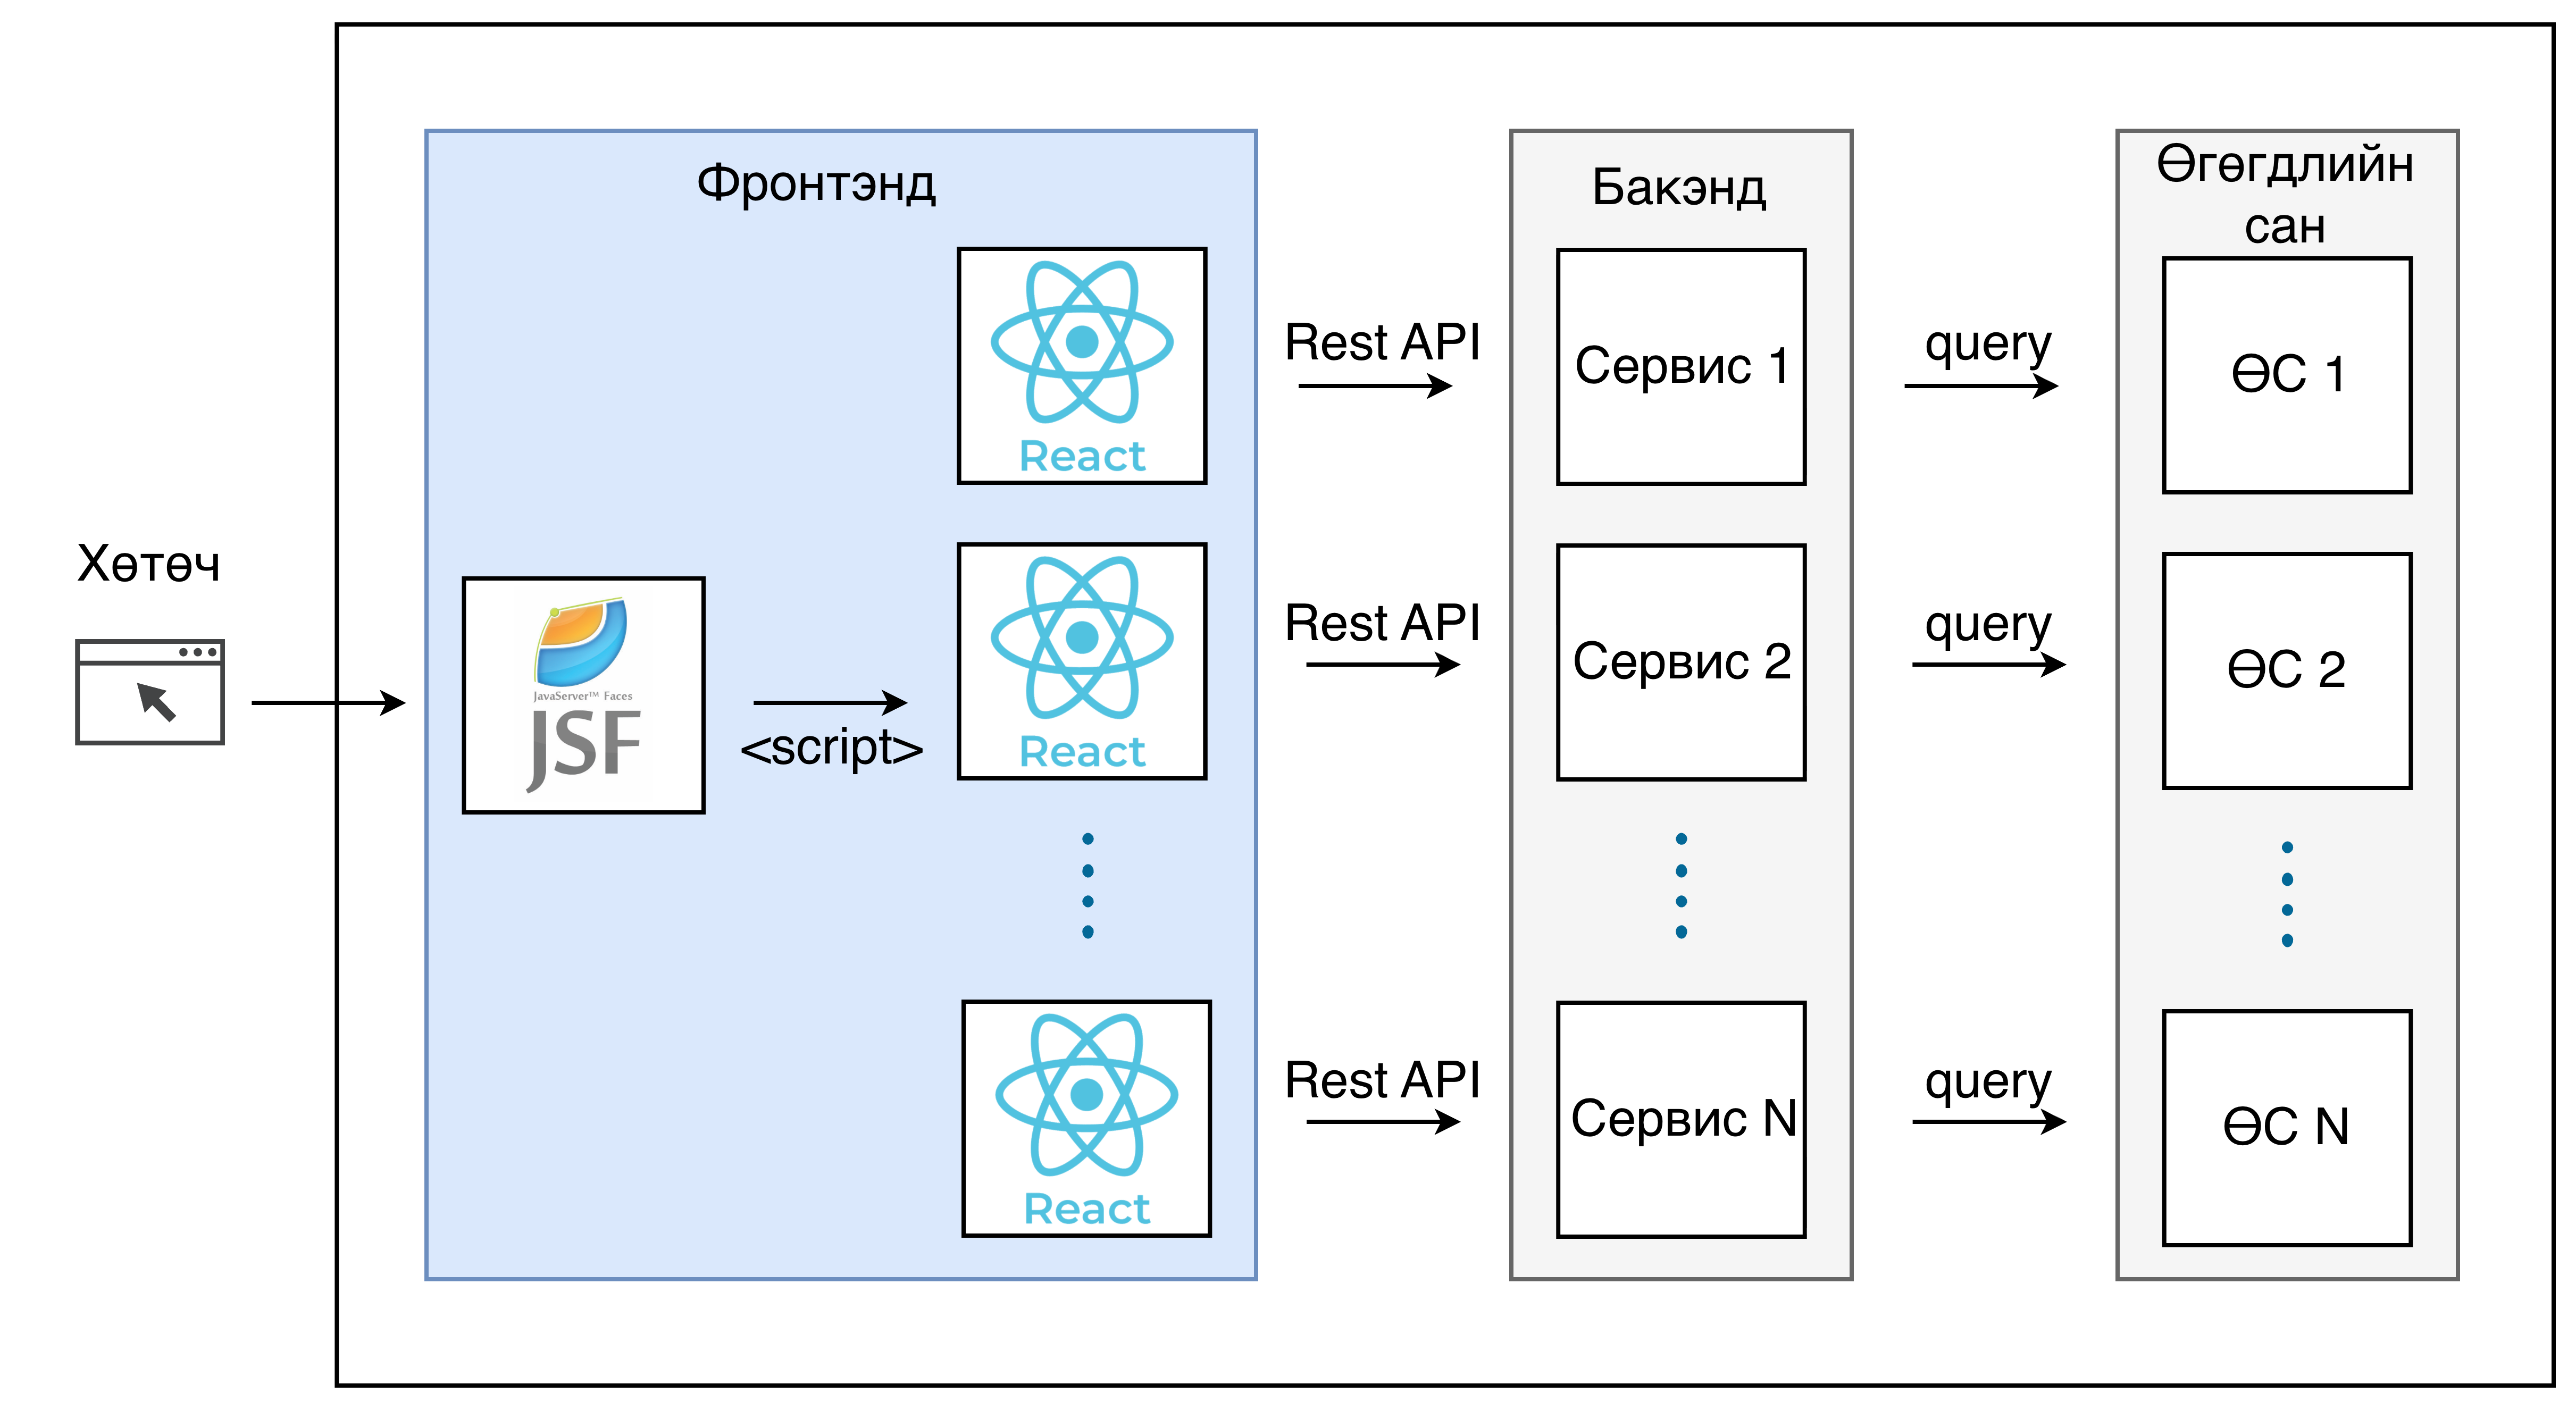
\includegraphics[width=14cm]{images/hybrid-mfe.png}
  \caption{Санал болгож буй холимог микрофронтенд архитектурын шийдэл}
  \label{fig:hybrid-mfe}
\end{figure}

% \subsection{UI/UX зохиомж}
% Микрофронтенд модулиуд нь кодын түвшинд тусдаа бие даан хөгжүүлэгддэг хэдий ч, эцсийн хэрэглэгчид нэгдмэл, цогц систем мэт харагдах шаардлагатай. Иймд кодын хэрэгжүүлэлтээс өмнө Figma платформ ашиглан системийн хэрэглэгчийн интерфейс (UI) болон хэрэглэгчийн туршлага (UX)-ын нэгдсэн загварыг боловсруулсан.

% \begin{figure}[H]
%   \centering
%   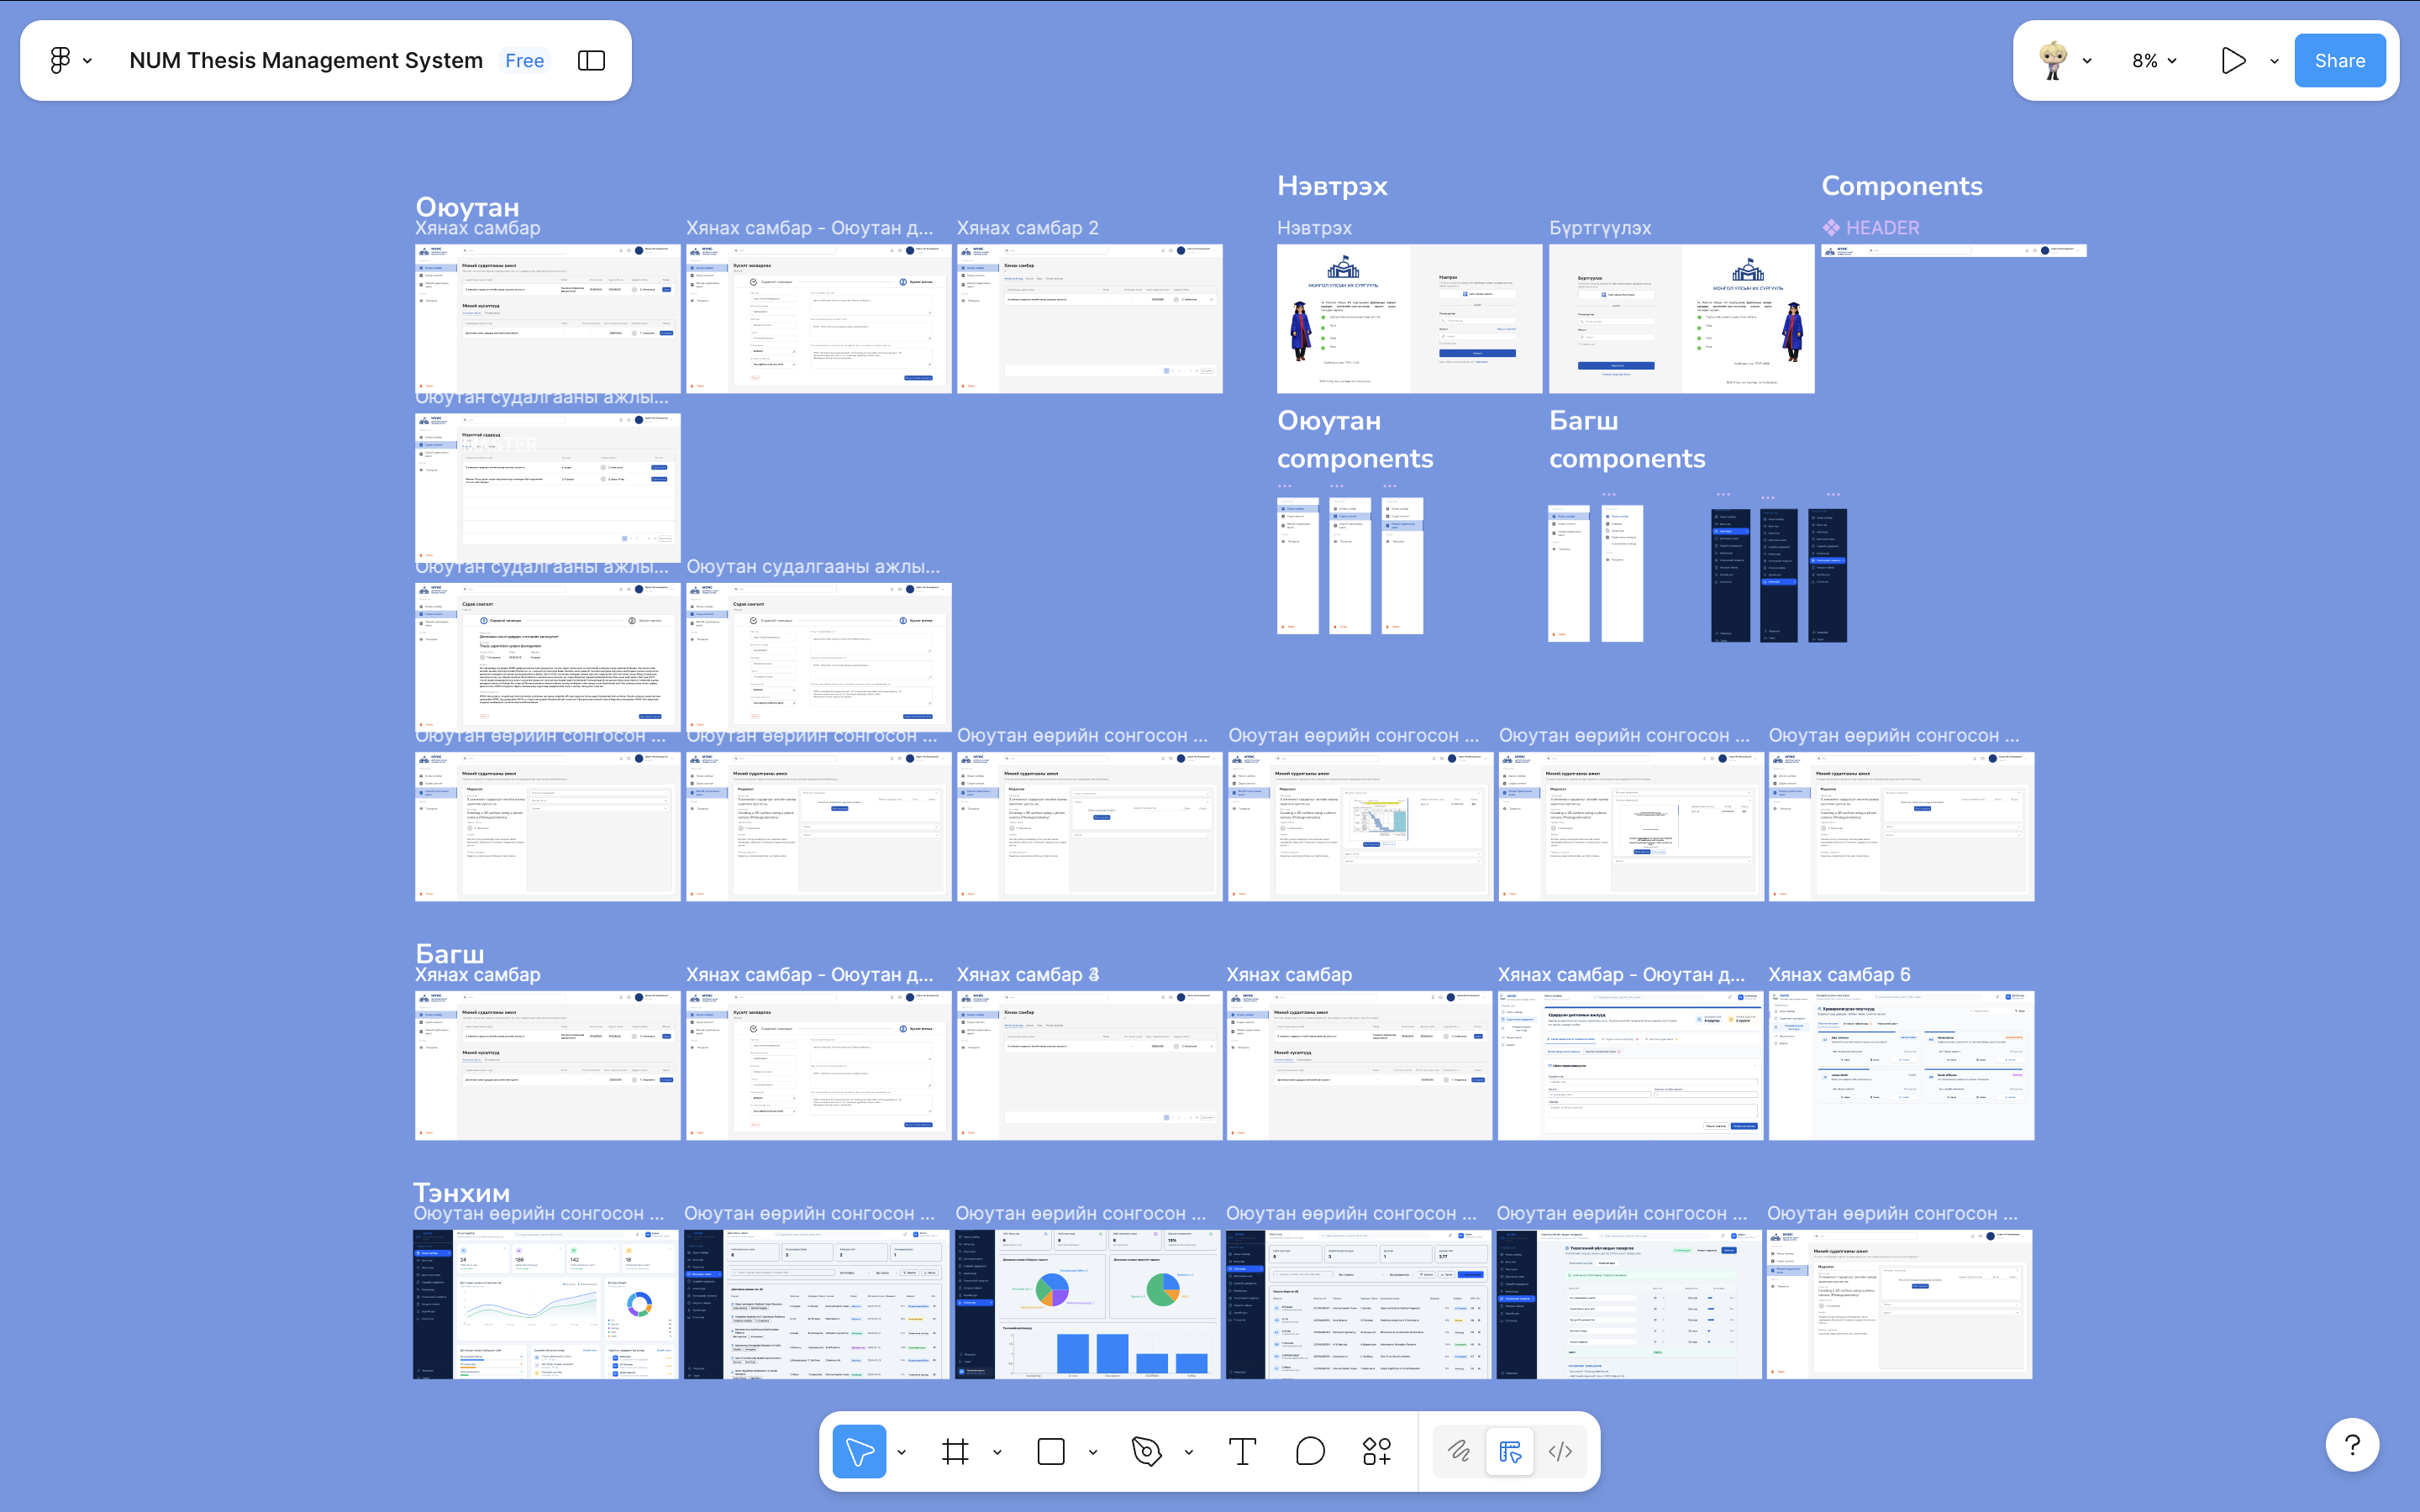
\includegraphics[width=16cm]{images/figma.png}
%   \caption{Figma дээр боловсруулсан системийн UI/UX загварын хэсэг}
%   \label{fig:figma}
% \end{figure}